\section{Modelo de dados}

Uma das componentes importantes do desenho de um sistema de informação, passa por criar um modelo que explique as características de funcionamento e comportamento do \textit{software} a ser desenvolvido. A modulação para além de ajudar na compreensão do sistema, evita erros de programação, de projeto e de funcionamento.

\subsection{Modelo de Domínio}

Um dos primeiros passos na planificação do sistema passou pela definição do \textbf{Modelo de Domínio}.
Pode-se classificar como domínio do sistema, o conjunto de características que descrevem a família de problemas que a aplicação pretende solucionar.

Pode-se consultar na Figura ~\ref{fig:modelo-dominio} os termos do sistema e as relações existentes entre esses termos.

\begin{figure}[H] 
  \centering
  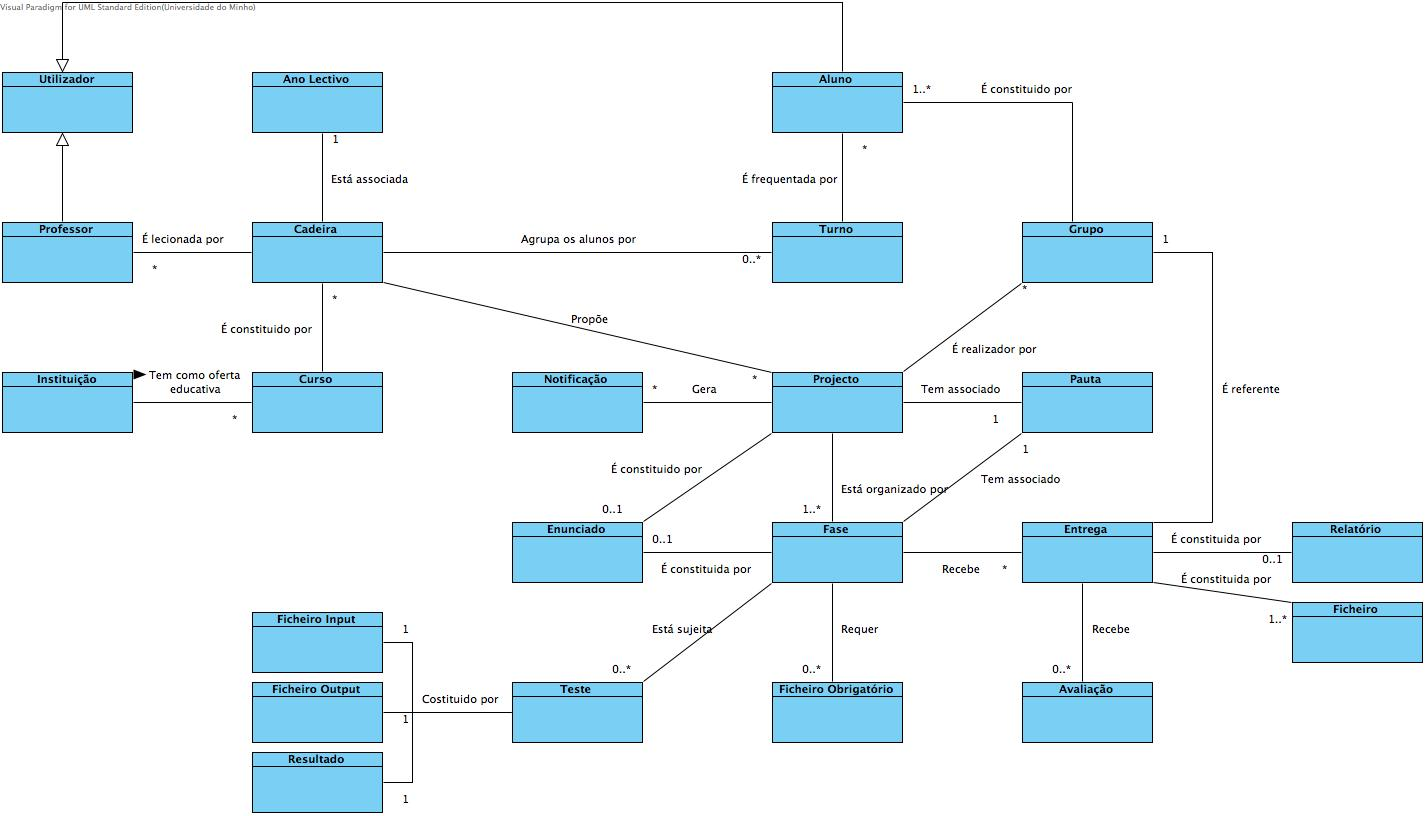
\includegraphics[width=1\textwidth,center]{images/modelo_dados/modelo-dominio}
  \caption{Modelo de domínio}
  \label{fig:modelo-dominio}
\end{figure}

\subsection{Diagrama de Classes}

Para representar a estrutura e relações das classes que servirão de modelo para os objetos do sistema, utilizaremos um \textbf{Diagrama de Classes}. Os diagramas de Classes são extremamente úteis para o desenvolvimento de sistemas, pois definem todas as classes que irão constituir o sistema e são uma excelente base para outras fases de planeamento e para o desenvolvimento.

Este tipo de diagramas permitem verificar como cada classe se relaciona com as outras, tendo como objetivo, a satisfação dos requisitos funcionais definidos para o sistema em estudo. 

Na Figura ~\ref{fig:diagrama-classes} podem-se ver representadas todas as classes e as suas relações que servirão como modelo para os objetos do sistema.

\begin{figure}[H] 
  \centering
  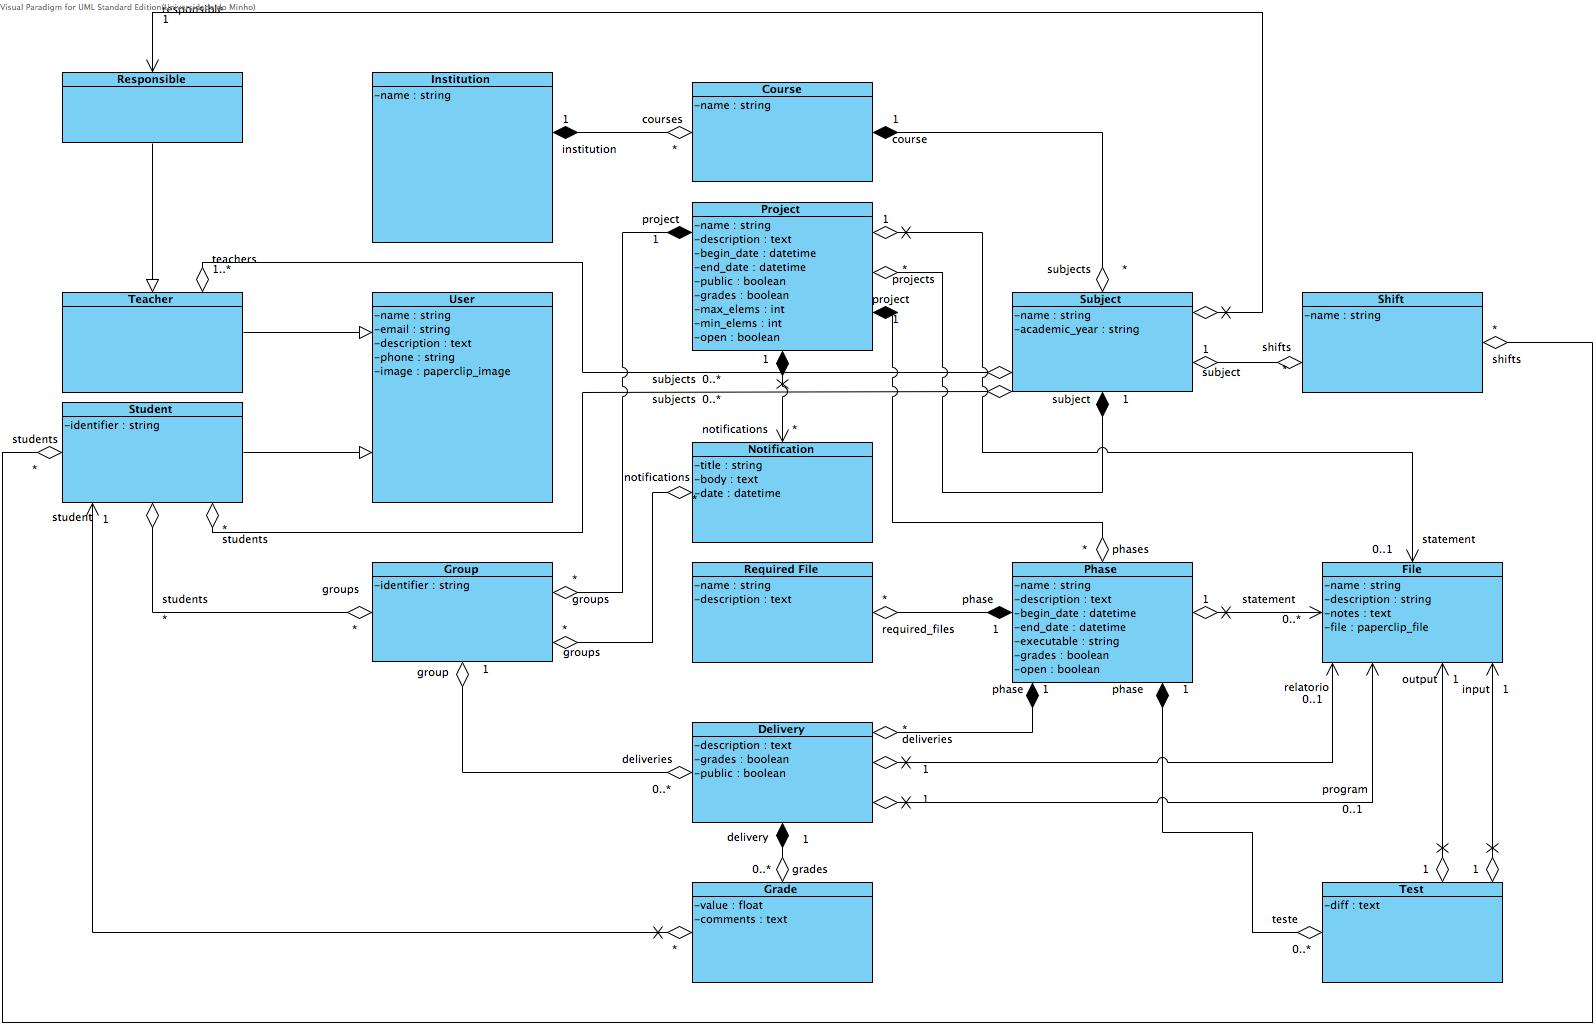
\includegraphics[width=1\textwidth,center]{images/modelo_dados/diagrama-classes}
  \caption{Diagrama de Classes}
  \label{fig:diagrama-classes}
\end{figure}

\subsection{Gramática Independente de Contexto}

Alternativamente ao Diagrama de Classes, definiu-se o sistema numa gramática independente de contexto na forma \textbf{Extended Backus-Naur(EBNF)}, representada de seguida:

\begin{spverbatim}
Institution : Course+ name=STRING 
            ;

Course : Subject+ name=STRING 
       ;

Subject : name=STRING academic_year=STRING Responsible Shift+ Teacher+ Student+ Project+ 
        ;

Project : name=STRING description=TEXT begin_date=DATETIME end_date=DATETIME public=BOOLEAN grades=BOOLEAN max_elems=INT min_elems=INT open=BOOLEAN Group+ Notification+ Phase+ statement=File?
        ;

Notification : title=STRING body=TEXT date=DATETIME Group+ 
             ;

Shift : name=STRING Subject Student* 
      ;

Phase : name=STRING description=TEXT begin_date=DATETIME end_date=DATETIME executable=STRING grades=BOOLEAN open=BOOLEAN File* statement=File? Required_File+ Delivery+ Test* 
      ;

File : name=STRING description=STRING notes=TEXT file=PAPERCLIP_FILE 
     ;

Test : diff=TEXT input=File output=File 
     ;

Required_File : name=STRING description=TEXT 
              ;

Delivery : description=TEXT grades=BOOLEAN public=BOOLEAN Grade* Group 
         ;

Grade : value=FLOAT comments=TEXT Student 
      ;

Group : identifier=STRING Notification+ Delivery* Student+ 
      ;

Student : User identifier=STRING Shift+ Group+ Subject+ 
        ;

Teacher : User Subject+ 
        ;

User : name=STRING email=STRING description=TEXT phone=STRING image=PAPERCLIP_FILE 
     ;

Responsible : Teacher 
            ;            
\end{spverbatim}

